%\title{Project Report}
%
%%% Preamble
\documentclass[paper=a4, fontsize=11pt]{scrartcl}
\usepackage[T1]{fontenc}
\usepackage{fourier}
\usepackage{listings}

\usepackage[english]{babel}															% English language/hyphenation
\usepackage[protrusion=true,expansion=true]{microtype}	
\usepackage{amsmath,amsfonts,amsthm} % Math packages
\usepackage[pdftex]{graphicx}	
\usepackage{url}
\usepackage{hyperref}
\usepackage{graphicx}
\usepackage{wrapfig}
\usepackage[margin=1.00in]{geometry}
\usepackage{amsmath}

%%% Custom sectioning
\usepackage{sectsty}
\allsectionsfont{\centering \normalfont\scshape}


%%% Custom headers/footers (fancyhdr package)
\usepackage{fancyhdr}
\pagestyle{fancyplain}
\fancyhead{}											% No page header
\fancyfoot[L]{}											% Empty 
\fancyfoot[C]{}											% Empty
\fancyfoot[R]{\thepage}									% Pagenumbering
\renewcommand{\headrulewidth}{0pt}			% Remove header underlines
\renewcommand{\footrulewidth}{0pt}				% Remove footer underlines
\setlength{\headheight}{3.6pt}
\date{}


%%% Equation and float numbering
\numberwithin{equation}{section}		% Equationnumbering: section.eq#
\numberwithin{figure}{section}			% Figurenumbering: section.fig#
\numberwithin{table}{section}				% Tablenumbering: section.tab#


%%% Maketitle metadata
\newcommand{\horrule}[1]{\rule{\linewidth}{#1}} 	% Horizontal rule

\title{
		\vspace{-1in} 	
		\usefont{OT1}{bch}{b}{n}
		\normalfont \normalsize \textsc{Durham Computer Science} \\ [5pt]
		\horrule{0.5pt} \\[0.4cm]
		\large  Optimisation Assignment - LLLL76\\
		\horrule{2pt} \\[0.5cm]
		\vspace{-1in} 	
}

%%% Begin document
\begin{document}
\maketitle
%%%%%%%%%%%%%%%%%%%%%%%%%%%%%%%%%%%%%%%%%%%%%%%%%%
\section*{Question One}
\subsection*{Part One}

Maximise:
\[-x_1 + 10 * x_2 \]
Subject to:
\[ x_1 + x_2 <= 10  \]
\[ -2x_1 + 3x_2 >= 12  \]
\[ 2x_1 + 3x_2 >= 18  \]
\[ x_2 <= 6  \]
\[ x_1 >= 0  \]
Where $ x_1 = X $ and $ x_2 = Y $

\begin{figure}[h]
\centering
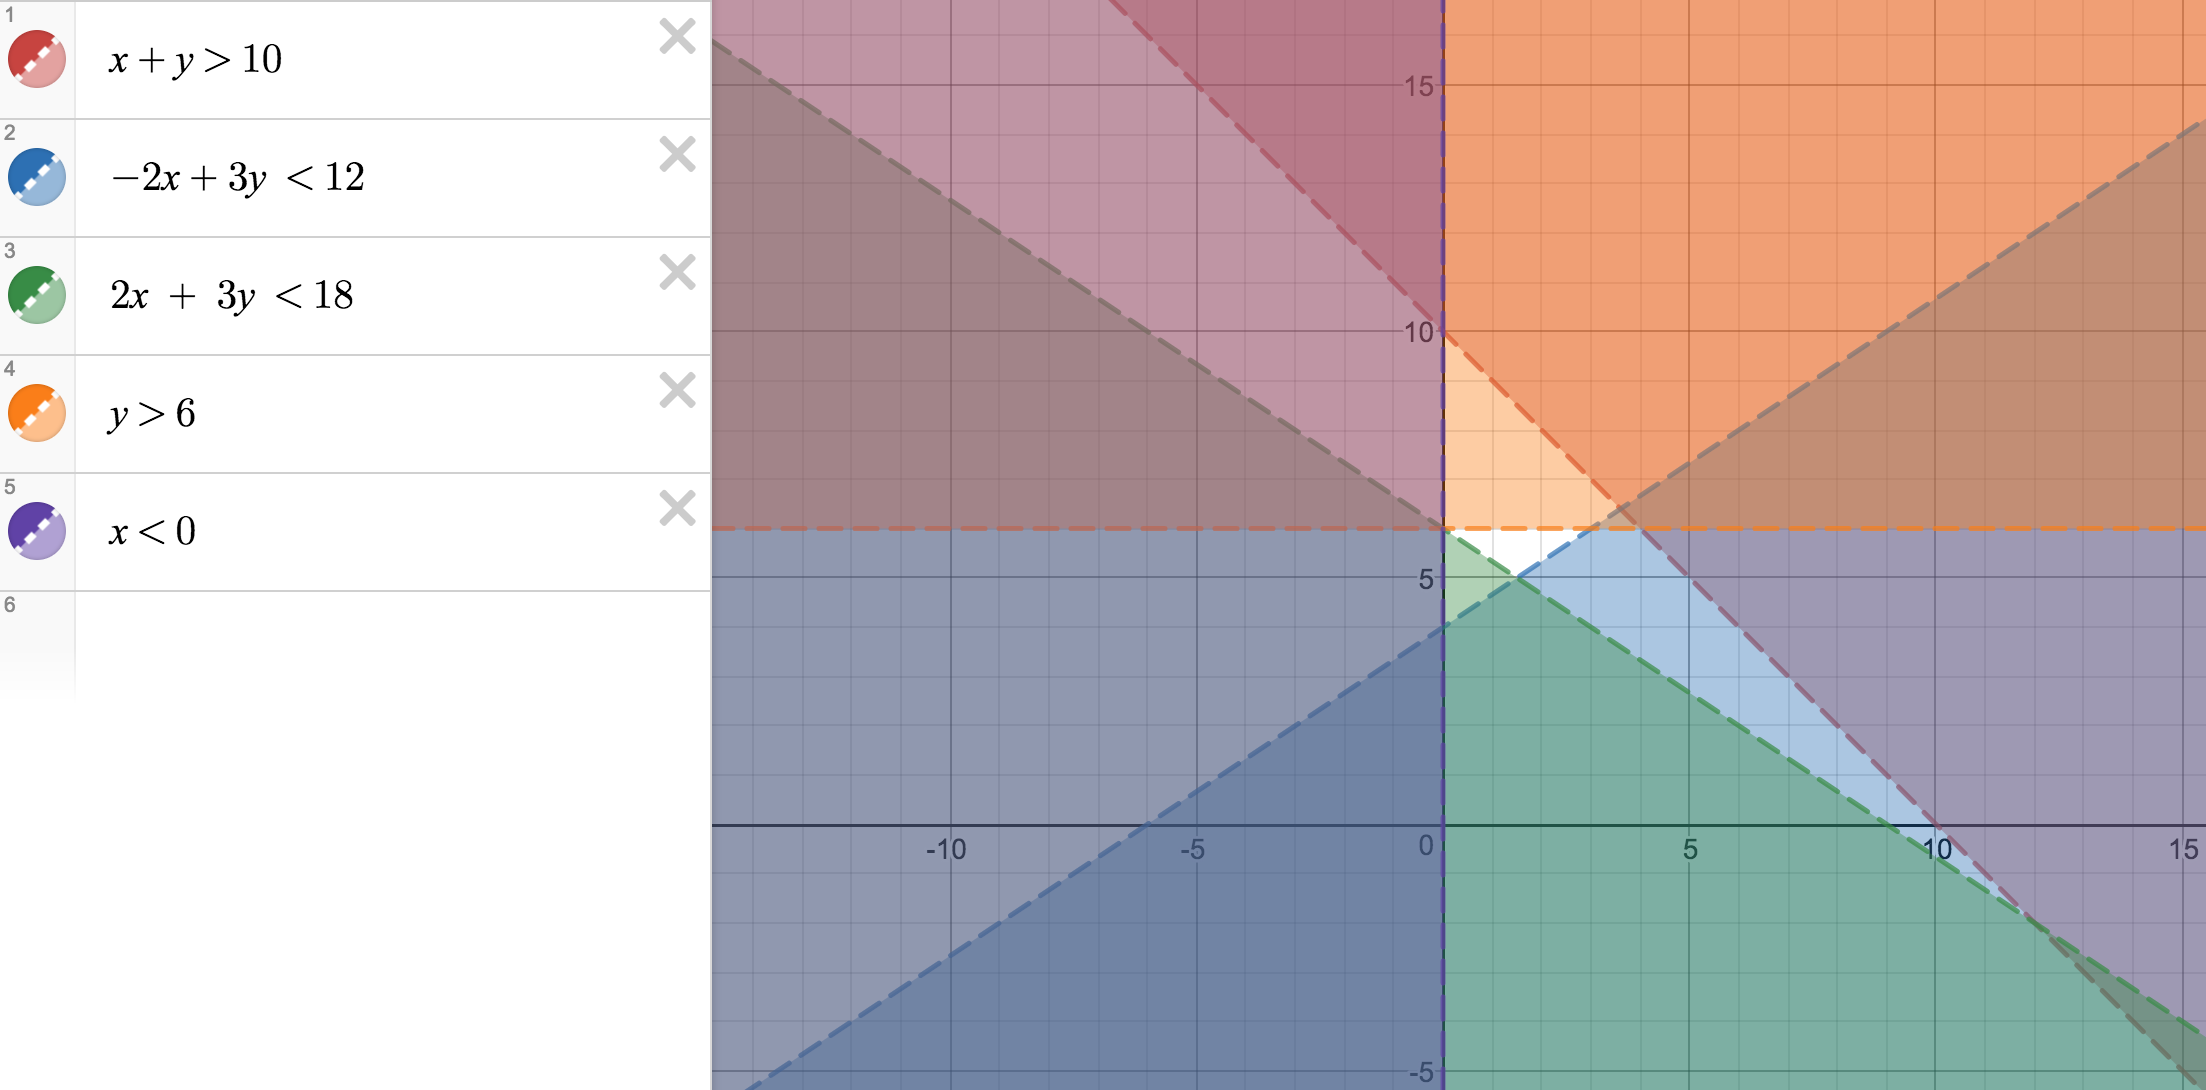
\includegraphics[width=\textwidth]{one_one.png}
\end{figure}

\subsection*{Part Two}

If:
\[ X + Y <= 10 \]
\[ -2X + 3Y >= 12 \]
\[ X >= 0 \]
are removed from the graph or:
\[ x_1 + x_2 <= 10  \]
\[ -2x_1 + 3x_2 >= 12  \]
\[ x_1 >= 0  \]
is removed from the question, then the optimal solution will remain the same.

\subsection*{Part Three}

\[ x_1 + x_2^+ - x_2^- + x_3 = 10 \]
\[ -2x_1 + 3x_2^+ - 3x_2^- - x_4 = 12 \]
\[ 2x_1 + 3x_2^+ - 3x_2^- -x_5 = 18 \]
\[ x_2^+ - x_2^- + x_6 = 6 \]

\[ x_1, x_2^+, x_2^-, x_3, x_4, x_5, x_6 >= 0 \]

%%%%%%%%%%%%%%%%%%%%%%%%%%%%%%%%%%%%%%%%%%%%%%%%%%
%%% End document
\end{document}